\documentclass[paper=a4, fontsize=11pt]{scrartcl}
\usepackage[T1]{fontenc}
\usepackage[utf8]{inputenc}
\usepackage{lmodern}
\usepackage{multirow}
\usepackage[table,xcdraw]{xcolor}
\usepackage[spanish]{babel}
\usepackage{cite}
\usepackage{amsmath,amsfonts,amsthm} % Math packages
\usepackage{graphics,graphicx, float} %para incluir imágenes y colocarlas
\usepackage[backref,colorlinks=true,linkcolor=black,urlcolor=blue,citecolor=blue]{hyperref} %Para crear enlaces en el pdf
\usepackage{url}
\usepackage[shortlabels]{enumitem}
\usepackage{appendix}
\usepackage{eurosym}
\usepackage{epsfig}
\usepackage{caption}
\usepackage{subcaption}

\usepackage{xcolor}
\usepackage{framed}
\definecolor{shadecolor}{RGB}{239, 251, 255}

\usepackage{listings}
\usepackage{color}

\definecolor{dkgreen}{rgb}{0,0.6,0}
\definecolor{gray}{rgb}{0.5,0.5,0.5}
\definecolor{mauve}{rgb}{0.58,0,0.82}
\definecolor{lgrey}{rgb}{0.9,0.9,0.9}


\lstset{frame=tb,
  language=C++,
  aboveskip=3mm,
  belowskip=3mm,
  showstringspaces=false,
  columns=flexible,
  basicstyle={\small\ttfamily},
  numbers=none,
  numberstyle=\tiny\color{gray},
  keywordstyle=\color{blue},
  commentstyle=\color{dkgreen},
  stringstyle=\color{mauve},
  breaklines=true,
  breakatwhitespace=true,
  tabsize=3
}

\renewcommand{\appendixname}{Anexo}
\renewcommand{\appendixtocname}{Anexo}
\renewcommand{\appendixpagename}{Anexo}

\numberwithin{figure}{section} % Number figures within sections (i.e. 1.1, 1.2, 2.1, 2.2 instead of 1, 2, 3, 4)
\numberwithin{table}{section} % Number tables within sections (i.e. 1.1, 1.2, 2.1, 2.2 instead of 1, 2, 3, 4)
\newcommand{\horrule}[1]{\rule{\linewidth}{#1}} % Create horizontal rule command with 1 argument of height

\title{
    \normalfont \normalsize
    \textsc{{\textbf{Algorítmica (2016-2017)}} \\ Grado en Ingeniería Informática \\ Universidad de Granada} \\ [25pt] % Your university, school and/or department name(s)
    \horrule{0.5pt} \\[0.4cm] % Thin top horizontal rule
    \huge Memoria Práctica 4: Backtracking y Branch & Bound\\ % The assignment title
    \horrule{2pt} \\[0.5cm] % Thick bottom horizontal rule
}
\author{Antonio de la Vega Jiménez }

%*************************************************************


\begin{document}

\maketitle % Muestra el Título
\newpage %inserta un salto de página
\tableofcontents % para generar el índice de contenidos
\listoffigures
\newpage

%*************************************************************

\section{Información PC usado}

\subsection{Hardware}
El hardware usado tiene las siguientes características:
\begin{itemize}
  \item \textbf{CPU:} \texttt{Intel(R) Core(TM) i3 CPU  540}
  \item \textbf{Velocidad reloj:} \texttt{3.07GHz}
  \item \textbf{Caché:} \texttt{4096 KB}
  \item \textbf{RAM:} \texttt{6040128 kB  }
\end{itemize}
\subsection{Software}
\subsubsection{Sistema operativo}
\begin{itemize}
  \item \textbf{SO:} \texttt{Manjaro Linux}
  \item \textbf{Kernel:}\texttt{ 4.4.52-1-MANJARO}
\end{itemize}
\subsubsection{Compilador}
\begin{itemize}
  \item \textbf{Versión compilador:} \texttt{g++ (GCC) 6.3.1 20170109}
\end{itemize}

\section{Algoritmos de ordenación básicos}

\subsection{Burbuja}
El código usado es el mostrado en la figura  \ref{fig1}

\begin{figure}[H]
        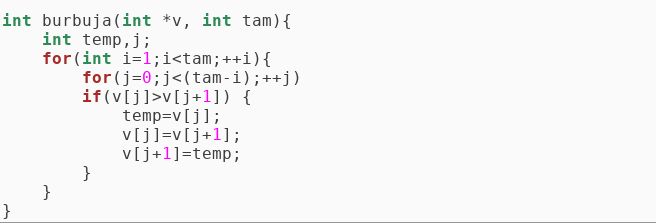
\includegraphics[scale=0.7]{imagenes/burbuja.png}
        \caption{Código burbuja.}
        \label{fig1}
\end{figure}

\subsubsection{Eficiencia teórica}

\begin{itemize}
  \item \textbf{Peor caso:} En el peor caso tendríamos lo siguiente:
  \begin{equation}
      \sum_{i=1}^{n}\sum_{j=0}^{n-1}14 = 14 n^2
  \end{equation}
  Por lo tanto tendremos eficiencia \begin{equation} O(n^2) \end{equation}
  
  \item \textbf{Caso mejor:} En el mejor caso la eficiencia es la misma.
  \item \textbf{Caso promedio:} En este caso se sigue manteniendo la misma eficiencia.
\end{itemize}

\subsubsection{Eficiencia empírica}

Al representar los datos obtenemos las siguientes gráfica:

\begin{figure}[H]
    \begin{center}
        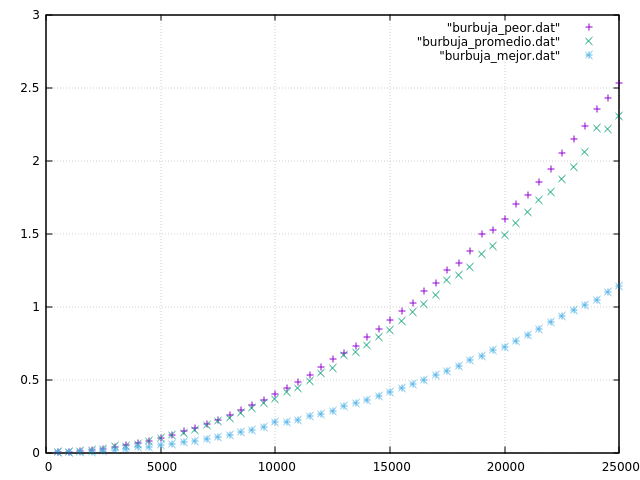
\includegraphics[scale=0.7]{imagenes/g_b.png}
        \caption{Tiempos de ejecución.}
        \label{fig2}
    \end{center}
\end{figure}

\subsubsection{Ajuste curva teórica a empírica}

En este paso realizamos el siguiente ajuste:
\begin{shaded*}
\begin{verbatim}
gnuplot> f(x) = a*x*x + b*x + c
gnuplot> fit f(x) "burbuja_peor.dat" via a,b,c
\end{verbatim}
\end{shaded*}

De forma que obtenemos los siguiente parámetros:

\begin{shaded*}
\begin{verbatim}
Final set of parameters            Asymptotic Standard Error
=======================            ==========================
a               = 4.08133e-09      +/- 2.704e-11    (0.6626%)
b               = -9.2079e-07      +/- 7.113e-07    (77.25%)
c               = 0.00281239       +/- 0.003932     (139.8%)

correlation matrix of the fit parameters:
                a      b      c      
a               1.000 
b              -0.969  1.000 
c               0.760 -0.876  1.000 

\end{verbatim}
\end{shaded*}

Y finalmente obtenemos la siguiente función ajustada:
\begin{figure}[H]
    \begin{center}
        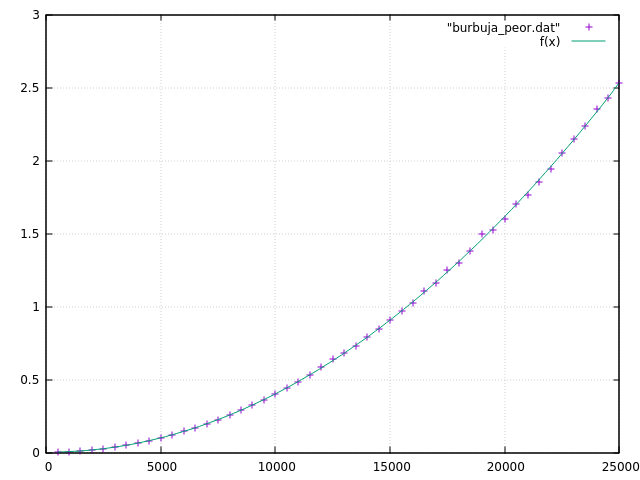
\includegraphics[scale=0.7]{imagenes/b_adj.png}
        \caption{Ajuste eficiencia teórica y empírica.}
        \label{fig3}
    \end{center}
\end{figure}

%*************************************
%*************************************
%*************************************
%*************************************

\subsection{Inserción}
El código usado es el mostrado en la figura  \ref{fig4}

\begin{figure}[H]
        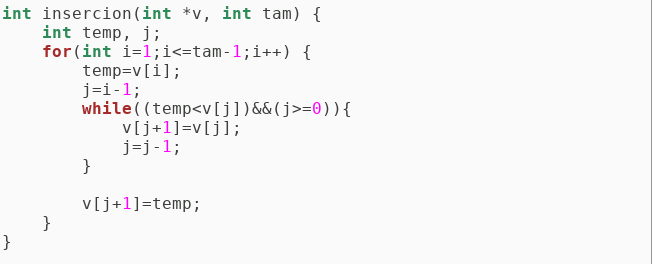
\includegraphics[scale=0.7]{imagenes/insercion.png}
        \caption{Código inserción.}
        \label{fig4}
\end{figure}

\subsubsection{Eficiencia teórica}

\begin{itemize}
  \item \textbf{Peor caso:} En el peor caso tendríamos lo siguiente:
  \begin{equation}
      \sum_{i=1}^{n} \sum_{j=i-1}^{0} 6 + 8 
  \end{equation}
  Por lo tanto tendremos eficiencia \begin{equation} O(n^2) \end{equation}
  
  \item \textbf{Caso mejor:} En el mejor caso no se recorre nunca el bucle while, por lo que la eficiencia será \begin{equation} \Omega(n) \end{equation} .
  \item \textbf{Caso promedio:} En este caso se obtiene la misma eficiencia que en el peor caso ya que si se entrará en el while aunque sean menos veces.
\end{itemize}

\subsubsection{Eficiencia empírica}

Al representar los datos obtenemos las siguientes gráfica:

\begin{figure}[H]
    \begin{center}
        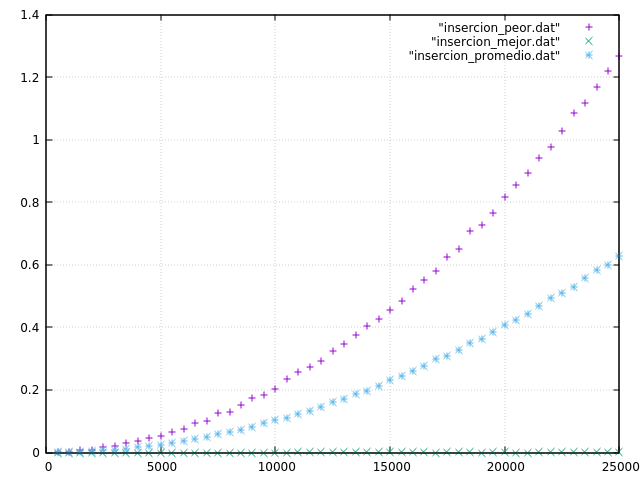
\includegraphics[scale=0.7]{imagenes/g_i.png}
        \caption{Tiempos de ejecución (los del mejor caso son demasiado pequeños para mostrarse correctamente).}
        \label{fig5}
    \end{center}
\end{figure}

\subsubsection{Ajuste curva teórica a empírica}

En este paso realizamos el siguiente ajuste:
\begin{shaded*}
\begin{verbatim}
gnuplot> f(x) = a*x*x + b*x + c
gnuplot> fit f(x) "insercion_peor.dat" via a,b,c
\end{verbatim}
\end{shaded*}

De forma que obtenemos los siguientes parámetros:

\begin{shaded*}
\begin{verbatim}
Final set of parameters            Asymptotic Standard Error
=======================            ==========================
a               = 2.00951e-09      +/- 1.448e-11    (0.7204%)
b               = 3.21917e-07      +/- 3.808e-07    (118.3%)
c               = 0.00297364       +/- 0.002105     (70.78%)

correlation matrix of the fit parameters:
                a      b      c      
a               1.000 
b              -0.969  1.000 
c               0.760 -0.876  1.000 

\end{verbatim}
\end{shaded*}

Y finalmente obtenemos la siguiente función ajustada:
\begin{figure}[H]
    \begin{center}
        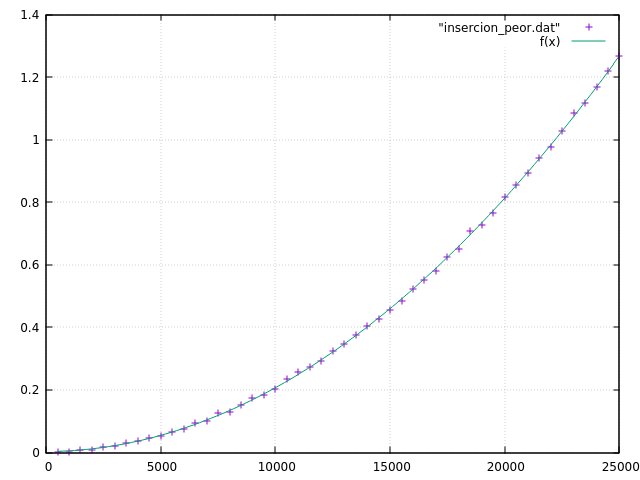
\includegraphics[scale=0.7]{imagenes/i_adj.png}
        \caption{Ajuste eficiencia teórica y empírica.}
        \label{fig6}
    \end{center}
\end{figure}


%*************************************
%*************************************
%*************************************
%*************************************

\subsection{Selección}
El código usado es el mostrado en la figura  \ref{fig7}

\begin{figure}[H]
        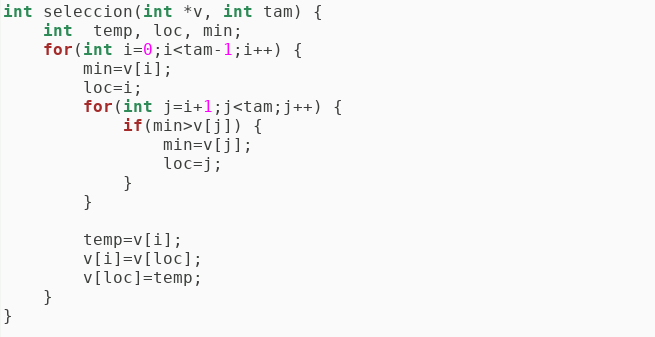
\includegraphics[scale=0.7]{imagenes/seleccion.png}
        \caption{Código selección.}
        \label{fig7}
\end{figure}

\subsubsection{Eficiencia teórica}

\begin{itemize}
  \item \textbf{Peor caso:} En el peor caso tendríamos lo siguiente:
  \begin{equation}
      \sum_{i=0}^{n-1} \sum_{j=i+1}^{n} 10 + 5 = 15n^2
  \end{equation}
  Por lo tanto tendremos eficiencia \begin{equation} O(n^2) \end{equation}
  
  \item \textbf{Caso mejor:} En el mejor caso también se recorren los dos bucles por lo que se tiene la misma eficiencia que en el peor caso.
  \item \textbf{Caso promedio:} Al igual que en el caso mejor, se obtiene la misma eficiencia que en el caso peor.
\end{itemize}

\subsubsection{Eficiencia empírica}

Al representar los datos obtenemos las siguientes gráfica:

\begin{figure}[H]
    \begin{center}
        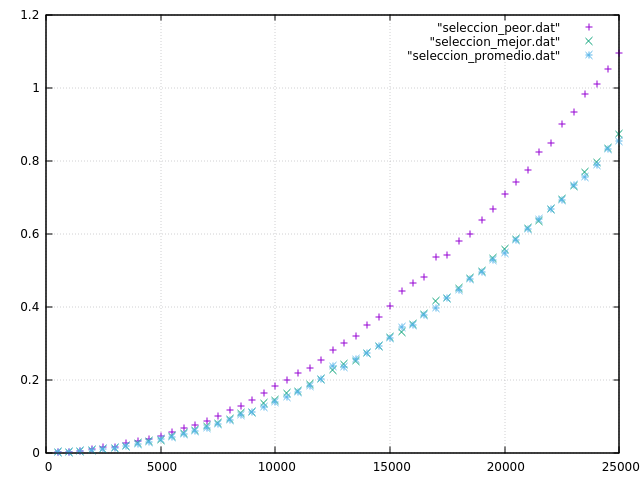
\includegraphics[scale=0.7]{imagenes/g_s.png}
        \caption{Tiempos de ejecución (los del mejor caso son demasiado pequeños para mostrarse correctamente).}
        \label{fig8}
    \end{center}
\end{figure}

\subsubsection{Ajuste curva teórica a empírica}

En este paso realizamos el siguiente ajuste:
\begin{shaded*}
\begin{verbatim}
gnuplot> f(x) = a*x*x + b*x + c
gnuplot> fit f(x) "seleccion_peor.dat" via a,b,c
\end{verbatim}
\end{shaded*}

De forma que obtenemos los siguiente parámetros:

\begin{shaded*}
\begin{verbatim}
Final set of parameters            Asymptotic Standard Error
=======================            ==========================
a               = 1.72138e-09      +/- 1.702e-11    (0.9885%)
b               = 1.04238e-06      +/- 4.476e-07    (42.94%)
c               = -0.00176612      +/- 0.002474     (140.1%)

correlation matrix of the fit parameters:
                a      b      c      
a               1.000 
b              -0.969  1.000 
c               0.760 -0.876  1.000 

\end{verbatim}
\end{shaded*}

Y finalmente obtenemos la siguiente función ajustada:
\begin{figure}[H]
    \begin{center}
        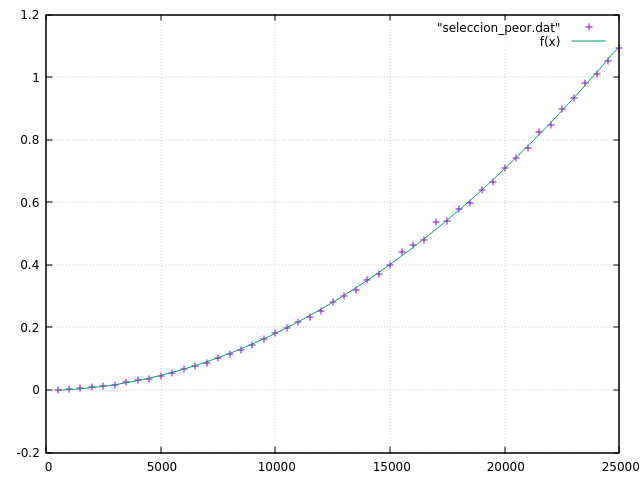
\includegraphics[scale=0.7]{imagenes/s_adj.png}
        \caption{Ajuste eficiencia teórica y empírica.}
        \label{fig9}
    \end{center}
\end{figure}


%*************************************
%*************************************
%*************************************
%*************************************

\section{Algoritmos de Ordenación con estructuras jerárquicas}

\subsection{Árbol binario de búsqueda}
El código usado es el mostrado en la figura  \ref{fig18}

\begin{figure}[H]
        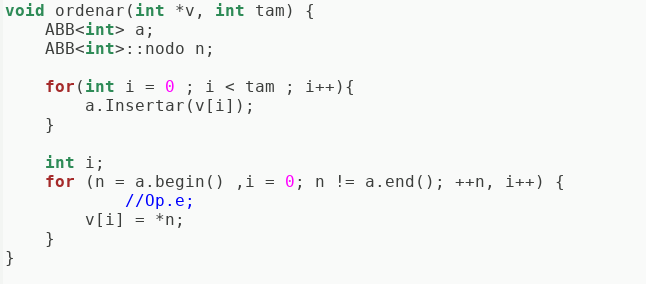
\includegraphics[scale=0.7]{imagenes/abb.png}
        \caption{Código ABB.}
        \label{fig18}
\end{figure}

\subsubsection{Eficiencia teórica}

\begin{itemize}
  \item \textbf{Peor caso:} Añadir un elemento a un árbol binario de búsqueda en el peor caso (si no está balanceado) es O(n) por lo cual la eficiencia para añadir n elementos será:
  \begin{equation} O(n^2) \end{equation}
  
  \item \textbf{Caso mejor:} En el mejor caso añadir un elemento a un árbol binario de búsqueda es de eficiencia logarítmica, por lo tanto añadir n elementos es: 
  \begin{equation} \Omega(n log_2n) \end{equation} 
  \item \textbf{Caso promedio:} En este caso se obtiene la misma eficiencia que en el mejor caso.
\end{itemize}

\subsubsection{Eficiencia empírica}

Al representar los datos obtenemos las siguientes gráfica:

\begin{figure}[H]
    \begin{center}
        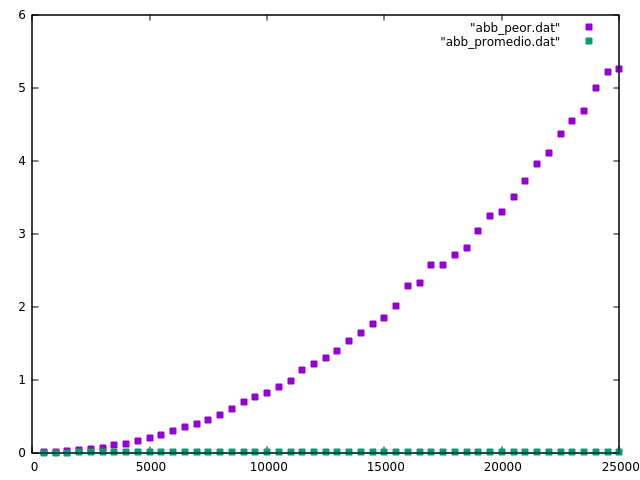
\includegraphics[scale=0.7]{imagenes/g_abb.png}
        \caption{Tiempos de ejecución (los del mejor caso son demasiado pequeños para mostrarse correctamente).}
        \label{fig19}
    \end{center}
\end{figure}

\subsubsection{Ajuste curva teórica a empírica}

En este paso realizamos el siguiente ajuste para el \textbf{peor caso}:
\begin{shaded*}
\begin{verbatim}
gnuplot> f(x) = a*x*x + b*x + c
gnuplot> fit f(x) "abb_peor.dat" via a,b,c

\end{verbatim}
\end{shaded*}

De forma que obtenemos los siguiente parámetros:

\begin{shaded*}
\begin{verbatim}
Final set of parameters            Asymptotic Standard Error
=======================            ==========================
a               = 8.78705e-09      +/- 1.354e-10    (1.541%)
b               = -6.43386e-06     +/- 3.562e-06    (55.36%)
c               = 0.0104211        +/- 0.01969      (188.9%)

correlation matrix of the fit parameters:
                a      b      c      
a               1.000 
b              -0.969  1.000 
c               0.760 -0.876  1.000 

\end{verbatim}
\end{shaded*}

Y finalmente obtenemos la siguiente función ajustada:
\begin{figure}[H]
    \begin{center}
        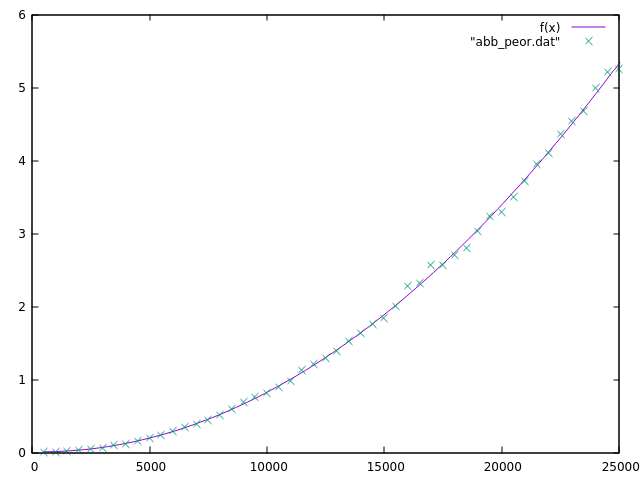
\includegraphics[scale=0.7]{imagenes/abb_adjp.png}
        \caption{Ajuste eficiencia teórica y empírica.}
        \label{fig20}
    \end{center}
\end{figure}

Ahora realizamos el siguiente ajuste para el \textbf{mejor caso o el promedio}:
\begin{shaded*}
\begin{verbatim}
gnuplot>  f(x) = a*x*(log(x)/log(2))
gnuplot> fit f(x) "abb_promedio.dat" via a

\end{verbatim}
\end{shaded*}

De forma que obtenemos los siguiente parámetros:

\begin{shaded*}
\begin{verbatim}
Final set of parameters            Asymptotic Standard Error
=======================            ==========================
a               = 3.63149e-08      +/- 3.959e-10    (1.09%)


\end{verbatim}
\end{shaded*}

Y finalmente obtenemos la siguiente función ajustada:
\begin{figure}[H]
    \begin{center}
        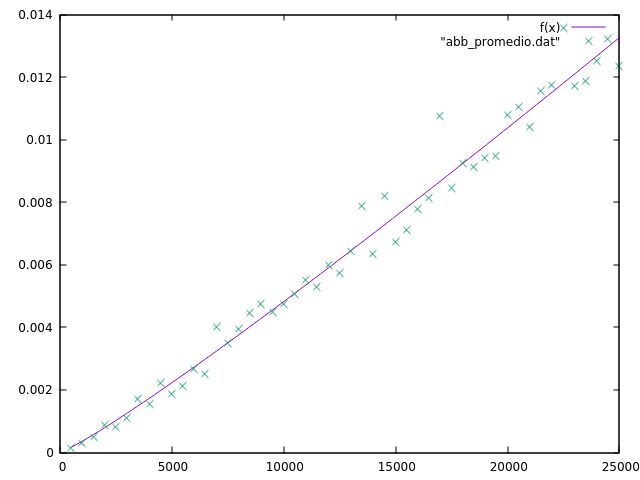
\includegraphics[scale=0.7]{imagenes/abb_adjm.png}
        \caption{Ajuste eficiencia teórica y empírica.}
        \label{fig21}
    \end{center}
\end{figure}

%*************************************
%*************************************
%*************************************
%*************************************
\subsection{Árbol parcialmente ordenado}
El código usado es el mostrado en la figura  \ref{fig21}

\begin{figure}[H]
        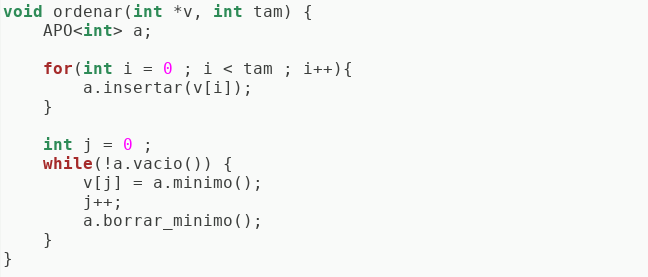
\includegraphics[scale=0.7]{imagenes/apo.png}
        \caption{Código APO.}
        \label{fig21}
\end{figure}

\subsubsection{Eficiencia teórica}

\begin{itemize}
  \item \textbf{Peor caso:} La eficiencia vale:
  \begin{equation} O(n \log_2n ) \end{equation}
  ya que se necesitan n operaciones de borrado de la raíz y reordenar el árbol tiene eficiencia logarítmica.
  \item \textbf{Caso mejor:} En este caso deberemos realizar las mismas operaciones por lo que la eficiencia es la misma.
  \item \textbf{Caso promedio:} Al igual que en caso mejor la eficiencia es igual a la del caso peor.
\end{itemize}

\subsubsection{Eficiencia empírica}

Al representar los datos obtenemos las siguientes gráfica:

\begin{figure}[H]
    \begin{center}
        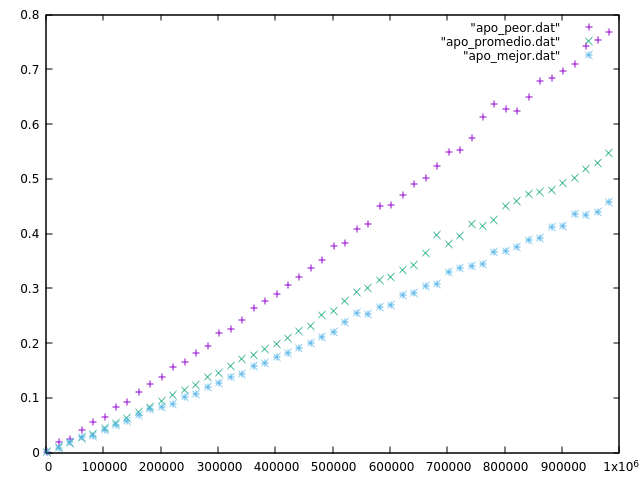
\includegraphics[scale=0.7]{imagenes/g_apo.png}
        \caption{Tiempos de ejecución.}
        \label{fig22}
    \end{center}
\end{figure}

\subsubsection{Ajuste curva teórica a empírica}

En este paso realizamos el siguiente ajuste:
\begin{shaded*}
\begin{verbatim}
gnuplot> f(x) = a*x*(log(x)/log(2))
gnuplot> fit f(x) "apo_peor.dat" via a
\end{verbatim}
\end{shaded*}

De forma que obtenemos los siguiente parámetros:

\begin{shaded*}
\begin{verbatim}

Final set of parameters            Asymptotic Standard Error
=======================            ==========================
a               = 4.02452e-08      +/- 1.887e-10    (0.4689%)

\end{verbatim}
\end{shaded*}

Y finalmente obtenemos la siguiente función ajustada:
\begin{figure}[H]
    \begin{center}
        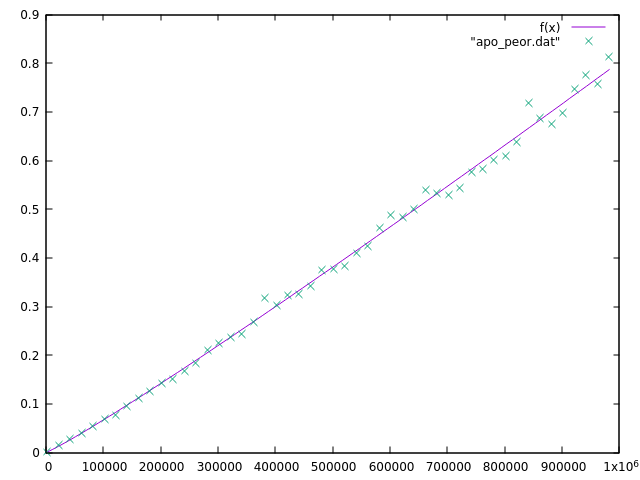
\includegraphics[scale=0.7]{imagenes/apo_adj.png}
        \caption{Ajuste eficiencia teórica y empírica.}
        \label{fig23}
    \end{center}
\end{figure}


%*************************************
%*************************************
%*************************************
%*************************************
\section{Algoritmo de Ordenación: fuerza bruta}

\subsection{Permutación}
El código usado es el mostrado en la figura  \ref{fig14}

\begin{figure}[H]
        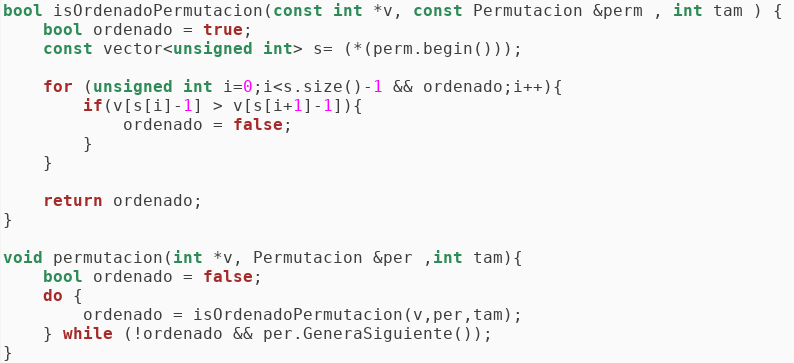
\includegraphics[scale=0.6]{imagenes/permutacion.png}
        \caption{Código permutación.}
        \label{fig14}
\end{figure}

\subsubsection{Eficiencia teórica}

\begin{itemize}
  \item \textbf{Peor caso:} En el peor caso tendríamos lo siguiente:
  Una eficiencia \begin{equation} O(n) \end{equation} para el algoritmo que comprueba si el vector está ordenado y una eficiencia \begin{equation} O(n!) \end{equation} para generar todas las permutaciones.
  Por lo tanto en el peor caso tendremos \begin{equation} O(n! n) \end{equation}
  
  \item \textbf{Caso mejor:} En el mejor caso solo habría que comprobar que el vector está ordenado, por lo que la eficiencia es \begin{equation} O(n) \end{equation} 
  \item \textbf{Caso promedio:} En este caso se obtiene la misma eficiencia que en el caso peor.
\end{itemize}

\subsubsection{Eficiencia empírica}

Al representar los datos obtenemos las siguientes gráfica:

\begin{figure}[H]
    \begin{center}
        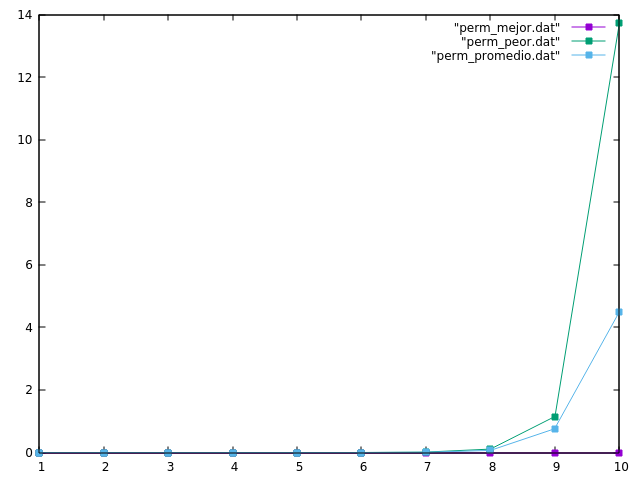
\includegraphics[scale=0.7]{imagenes/g_p.png}
        \caption{Tiempos de ejecución (los del mejor caso son demasiado pequeños para mostrarse correctamente).}
        \label{fig15}
    \end{center}
\end{figure}

\subsubsection{Ajuste curva teórica a empírica}

En este paso realizamos el siguiente ajuste:
\begin{shaded*}
\begin{verbatim}
gnuplot> fac(x) = (int(x)==0) ? 1.0 : int(x) * fac(int(x)-1.0)
gnuplot> f(x) = a*x*fac(x)
gnuplot> fit f(x) "perm_peor.dat" via a 
\end{verbatim}
\end{shaded*}

De forma que obtenemos los siguiente parámetros:

\begin{shaded*}
\begin{verbatim}
Final set of parameters            Asymptotic Standard Error
=======================            ==========================
a               = 3.7858e-07       +/- 8.047e-10    (0.2126%)

\end{verbatim}
\end{shaded*}

Y finalmente obtenemos la siguiente función ajustada:
\begin{figure}[H]
    \begin{center}
        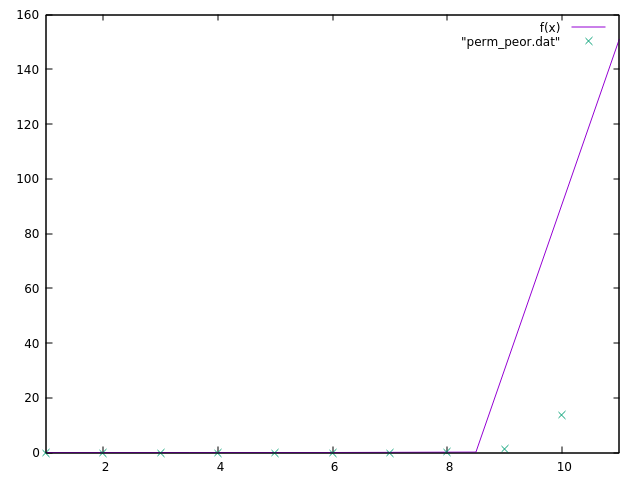
\includegraphics[scale=0.7]{imagenes/p_adj.png}
        \caption{Ajuste eficiencia teórica y empírica.}
        \label{fig16}
    \end{center}
\end{figure}

%*************************************
%*************************************
%*************************************
%*************************************
\section{Algoritmos de Ordenación por Mezcla}

\subsection{Mergesort}
El código usado es el mostrado en la figura  \ref{fig10}

\begin{figure}[H]
        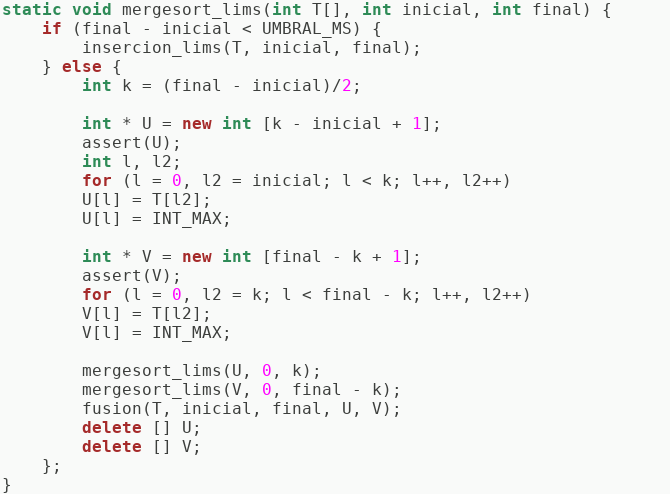
\includegraphics[scale=0.7]{imagenes/merge.png}
        \caption{Código mergesort.}
        \label{fig10}
\end{figure}

\subsubsection{Eficiencia teórica}
Vamos a suponer que el umbral usado es pequeño, en caso de usar un umbral muy grande la eficiencia seria la misma que la del algoritmo de ordenación por inserción.
\begin{itemize}
  \item \textbf{Peor caso:} En el peor caso tendríamos la siguiente eficiencia:
  \begin{equation} O(n \log_2n ) \end{equation} ya que se va dividiendo el vector por la mitad recursivamente.
  
  \item \textbf{Caso mejor:} En el mejor caso se tiene la misma eficiencia que en el peor caso.
  \item \textbf{Caso promedio:} Al igual que en el caso mejor, se obtiene la misma eficiencia que en el caso peor.
\end{itemize}

\subsubsection{Eficiencia empírica}

Al representar los datos obtenemos las siguientes gráfica:

\begin{figure}[H]
    \begin{center}
        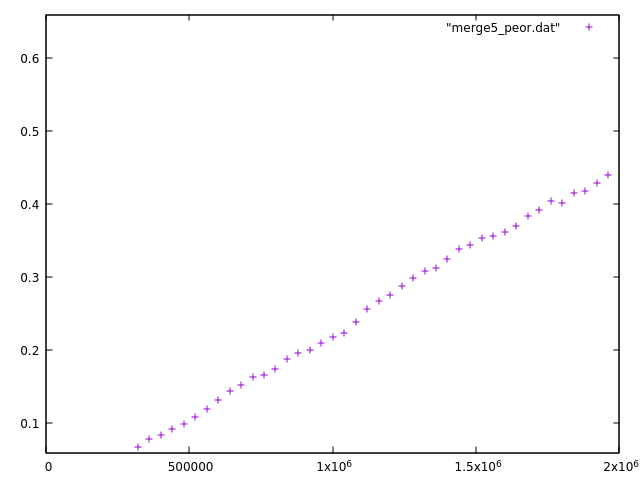
\includegraphics[scale=0.7]{imagenes/g_m.png}
        \caption{Tiempos de ejecución.}
        \label{fig11}
    \end{center}
\end{figure}

Al comprobar la evolución del algoritmo con diferentes umbrales (figura \ref{fig12}), podemos ver que cuanto más pequeño es el umbral, mejores tiempos se obtienen. El inconveniente de poner un umbral muy pequeño es que se hacen más llamadas recursivas y por lo tanto se puede llenar la pila con más facilidad.

\begin{figure}[H]
    \begin{center}
        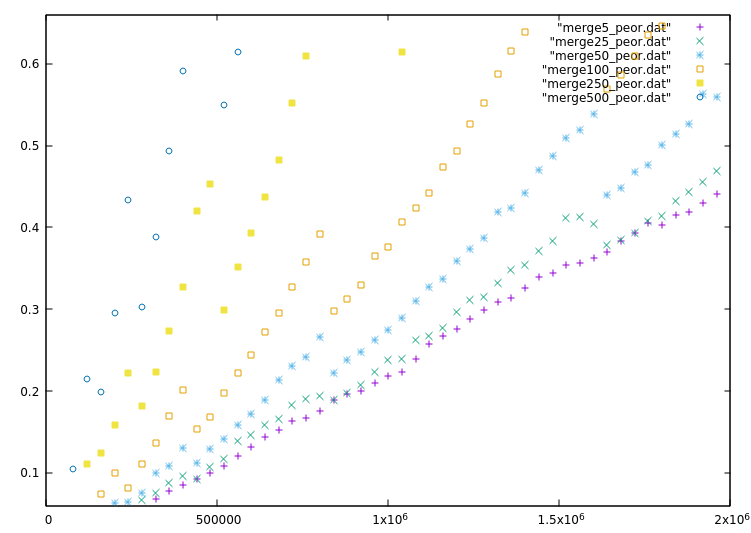
\includegraphics[scale=0.7]{imagenes/umbral.png}
        \caption{Tiempos de ejecución con diferentes umbrales}
        \label{fig12}
    \end{center}
\end{figure}

\subsubsection{Ajuste curva teórica a empírica}

En este paso realizamos el siguiente ajuste:
\begin{shaded*}
\begin{verbatim}
gnuplot> f(x) = a*x*(log(x)/log(2))
gnuplot> fit f(x) "merge5_peor.dat" via a

\end{verbatim}
\end{shaded*}

De forma que obtenemos los siguiente parámetros:

\begin{shaded*}
\begin{verbatim}
Final set of parameters            Asymptotic Standard Error
=======================            ==========================
a               = 1.10886e-08      +/- 4.188e-11    (0.3777%)

\end{verbatim}
\end{shaded*}

Y finalmente obtenemos la siguiente función ajustada:
\begin{figure}[H]
    \begin{center}
        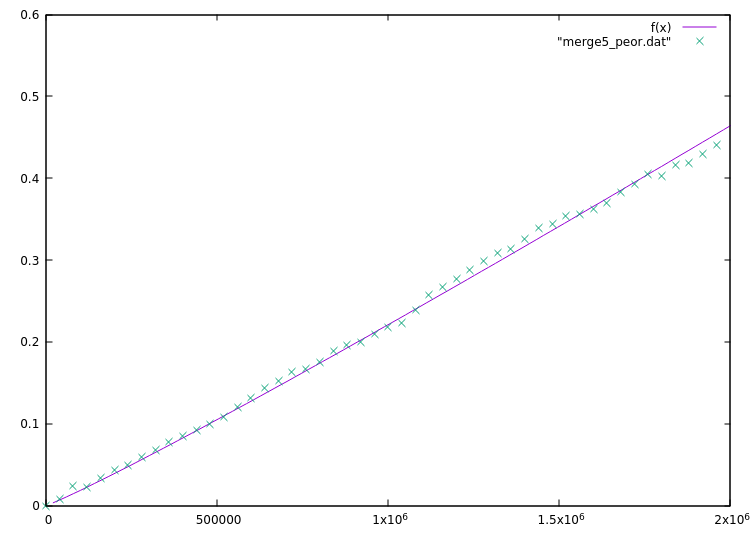
\includegraphics[scale=0.7]{imagenes/m_adj.png}
        \caption{Ajuste eficiencia teórica y empírica.}
        \label{fig13}
    \end{center}
\end{figure}


%*************************************************************
\newpage

\end{document}
